\section{Full Supporting Simulator Studies}
\label{app:holdout-details}
Study designs and explanatory passages are retained with their original
results. Selected definitions and results also appear in the main paper so
that its core comparison can be read independently.
\subsection{Supporting Study Design}

The independent v3 holdout compares a frozen DQL policy with deterministic
controls. The adverse-probe ablation holds that checkpoint fixed and varies
the promotion guard, using separate 30-seed inference and five-seed scale
cohorts. Expanded v4--v6 studies evaluate action coverage and contract changes;
they are development diagnostics, not additional holdout performance results.
Table~\ref{tab:action-contract-map} identifies these version boundaries.
Appendix~\ref{app:action-diagnostics} retains their detailed outcomes.

\begin{table}[!htbp]
\centering\small
\caption{Checkpoint, action-contract, and execution scope. A policy trained
under one action meaning is not evidence for another meaning.}
\Description{Rows separate legacy v3 performance, fixed-pool scale-out,
the rebalancing-only live trial, and the later cap-restoring development contract.}
\label{tab:action-contract-map}
\begin{tabular}{p{0.25\textwidth}p{0.29\textwidth}p{0.36\textwidth}}
\toprule
Study & Policy / action contract & Scope of the evidence\\
\midrule
v3 holdout and adverse-probe ablation & Frozen seed 101; legacy open-only scale-up & Reported rebalancing and multi-objective results; no cap-restoring claim\\
20,000-subscription scale-out & Same frozen checkpoint; fixed ten-connection pool & Endpoint migration; workload does not admit scaling actions\\
October loaded cluster trial & Same checkpoint; explicit rebalancing-only profile & Scaling actions disabled; three selective live migrations\\
v4--v5 development & Legacy scale-up; v5 corrects the scale-down guard & Action-coverage diagnostics; no selected holdout policy\\
v6 development & Versioned cap-restoring scale-up & Scripted action preflight and learner gates; no selected holdout policy\\
\bottomrule
\end{tabular}
\end{table}

The shared frozen deployment file has SHA-256 prefix
\texttt{3e68371d848eca85}; the reviewer evidence package retains the full hash
and weights. A missing contract field identifies the legacy checkpoint.
The current client permits it only for a compatible restricted action profile;
full-action deployment requires the versioned contract.

\subsection{Research Questions and Baselines}

The evaluation addresses four questions.  \textbf{RQ1} asks whether a frozen
DQL policy improves the multi-objective return and connection distribution
relative to a deterministic, two-dimensional heuristic.  \textbf{RQ2} asks
how the policy trades off the individual operating measurements alongside
the scalar reward. \textbf{RQ3} asks whether independently trained candidates use every allowed action in its
intended test scenario while respecting the fault guards.
\textbf{RQ4} asks whether rejecting an adverse probe promotion reduces the amount of queued work over time compared with overriding that
guard, blind promotion, static placement, and the guarded heuristic.

The v3 holdout compares three policies.  \emph{Static} retains the initial
transport assignment.  \emph{Heuristic} applies the threshold-based
subscription-count and backlog rules without value learning.  \emph{Frozen
DQL} uses the checkpoint selected on the fixed development-validation bank,
sets $\epsilon=0$, disables training, and invokes the same action masks and
execution guards as the deployed client.  The heuristic is the primary
baseline because it has the same rebalancing authority as DQL; the static
policy is the no-rebalancing control for the initial connection assignment.

During each episode, the policy receives only client-deployable observations:
local subscription queues, active-connection telemetry, interval throughput
counters, and one retained probe candidate.  Cluster-wide pod distributions are
calculated by the simulator only after an action for that interval has been
chosen.  They are evaluation outputs and are not inserted into the policy
state.  This maintains the partial-observability boundary formalized in
Section~\mainref{sec:problem-formulation}.

\subsection{Predeclared Protocol}

Patterson et al. identify hyperparameter selection, baseline construction,
and uncertainty reporting as central issues in empirical RL evaluation
\cite{Patterson2024EmpiricalDesign}. We therefore keep development selection
separate from the locked holdout and report component metrics alongside return.
Testing adaptation under changed execution conditions is also distinct from
measuring performance in the training setting, as demonstrated by Biagiola and
Tonella's plasticity analysis \cite{Biagiola2022Plasticity}. The operating and
fault scenarios below test this distinction without treating successful
training as evidence of universal adaptation.

Table~\ref{tab:locked-study-design} summarizes the evidence-generating runs.
In v3, three candidate networks were trained for exactly $10{,}000$
transitions under seeds 101, 211, and 307.  Candidate selection used ten fixed
validation seeds and required subscription-count rebalancing
($a^{\mathrm{reb}N}$), backlog rebalancing ($a^{\mathrm{reb}G}$), and full
connection migration ($a^{\mathrm{mig}}$) in at least $80\%$ of admissible
episodes in their intended scenarios.  Candidate 0 (seed 101) passed this gate
and was frozen before the holdout seed bank was read.

\begin{table}[!htbp]
  \caption{Locked simulator study design.  ``Not opened'' means that no
  performance episode was run on the reserved holdout seed bank.}
  \Description{Table comparing the v3 development run, v3 independent
  holdout, two v4 development runs, the v5 corrected-guard run, the v6
  action-contract preflight, and the v6 four-arm learner factorial by candidate
  count, transition budget, evaluation design, required gates, and holdout
  status, followed by the frozen-policy adverse-probe ablation.}
  \label{tab:locked-study-design}
  \centering
  \small
  \begin{tabular}{p{0.18\textwidth}p{0.15\textwidth}p{0.19\textwidth}p{0.23\textwidth}p{0.13\textwidth}}
    \toprule
    Study stage & Training budget & Fixed evaluation & Selection requirement & Holdout status \\
    \midrule
    v3 development & $3\times10{,}000$ transitions & 10 validation seeds; 4 scenarios & $a^{\mathrm{reb}N}$, $a^{\mathrm{reb}G}$, and $a^{\mathrm{mig}}$ each at $\geq80\%$ episode coverage & Not opened \\
    v3 holdout & Frozen seed 101; no updates & 10 new seeds; 4 scenarios; 3 policies; 120 episodes & No selection on holdout & Completed \\
    v4 uniform replay & $5\times20{,}000$ transitions & 10 validation seeds; 7 operating and 4 fault scenarios & All five intervention actions at $\geq80\%$, plus all safety guards & Not opened \\
    v4 stratified replay & $5\times20{,}000$ transitions & Same fixed v4 validation bank & Same all-action and safety gate & Not opened \\
    v5 corrected guard & $5\times20{,}000$ transitions & 10 fresh validation seeds; same 11 scenarios & Same all-action and safety gate & Not opened \\
    v6 scale-up preflight & No learner training & 10 paired seeds; 500 intervals & Target metric and reward improve for every seed, plus safety gates & Not defined \\
    v6 learner factorial & $4\times5\times20{,}000$ transitions & 10 fresh validation seeds; same 11 scenarios & At least 4/5 candidates pass every action and safety gate & Not defined \\
    Adverse-probe ablation & Frozen v3 checkpoint; no updates & 30 paired inference seeds and 5 paired 20k scale seeds; 500 intervals & Lower paired backlog AUC for guarded DQL than forced promotion & Completed \\
    \bottomrule
  \end{tabular}
\end{table}

The independent v3 holdout contains ten previously unused seeds for each of
four scenarios and 500 decision intervals per episode.  The connection-count
skew scenario uses 1,000 subscriptions; the tiered-backlog scenario uses 1,200
subscriptions; and the client-slowdown and pod-pressure-skew scenarios each use
1,600 subscriptions.  Every scenario has four modeled pods, four initial
persistent connections, and a maximum of six connections.  The tiered-backlog
scenario assigns $25\%$ of its queues to each initial backlog level
$100{,}000$, $50{,}000$, $5{,}000$, and zero.  The client-slowdown scenario
reduces acknowledgement capacity to $35\%$ of its nominal value between
intervals 125 and 375.  The other two scenarios isolate initial
subscription-count skew and the placement of three of four connections on one
pod, respectively.

For policy $\pi$, paired episode $j$, and metric $v$, let
$Y_{\pi,j,v}$ denote the episode mean.  We define a direction-adjusted paired
difference
\begin{equation}
  D_{j,v}=d_v\left(Y_{\mathrm{DQL},j,v}
  -Y_{\mathrm{base},j,v}\right),
  \qquad
  d_v=\begin{cases}
  +1,&\text{higher is better},\\
  -1,&\text{lower is better}.
  \end{cases}
  \label{eq:direction-adjusted-effect}
\end{equation}
Thus, a positive $D_{j,v}$ always favors DQL.  The relative benefit reported
below is
\begin{equation}
  \mathrm{RB}_v=100\,
  \frac{\overline{D}_v}{\left|\overline{Y}_{\mathrm{base},v}\right|}.
  \label{eq:relative-benefit}
\end{equation}
Overbars in these two equations denote means across paired episodes.
The metric index $v$ is distinct from the client-population size $m$.
We resample the 40 paired differences $10{,}000$ times to obtain percentile
$95\%$ confidence intervals.  Two-sided paired sign-flip tests are exact for
the scenario-level sets of ten pairs and use $100{,}000$ Monte Carlo sign
vectors for the pooled set of 40 pairs.  Pooled $p$-values are adjusted by the
Holm procedure across the complete family of 18 metric-by-baseline tests.  The
scenario box plots in Figure~\ref{fig:v3-scenario-reward} describe quartiles
and individual episode outcomes; the paired randomization tests
provide the statistical comparison.

We evaluate DQL as a sequential controller through return, operational
outcomes, paired effect sizes, and action coverage. Classifier accuracy and
ROC--AUC apply to labelled prediction tasks. Applying them here would mainly
measure agreement with a heuristic that supplied the correct-action labels,
rather than the controller's operating performance.

\subsection{Training Diagnostics and Frozen-Policy Selection}

Figure~\ref{fig:v3-training-diagnostics} shows the archived v3 development
traces. The upper panel reports the cumulative mean interval reward
$J^{-1}\sum_{\ell=1}^{J}R^{\mathrm{train}}_\ell$, where $J$ counts logged training
transitions and $R^{\mathrm{train}}_\ell$ is the recorded reward of transition $\ell$.
This is a mean, not accumulated reward, so its scale remains
comparable across checkpoints.  Candidate 0 recovered from the early
high-exploration regime and ended with the highest development mean
reward.  The other candidates follow similar but distinct trajectories, which
shows that the random seed has a clear effect on the learned values.

\begin{figure}[!htbp]
  \centering
  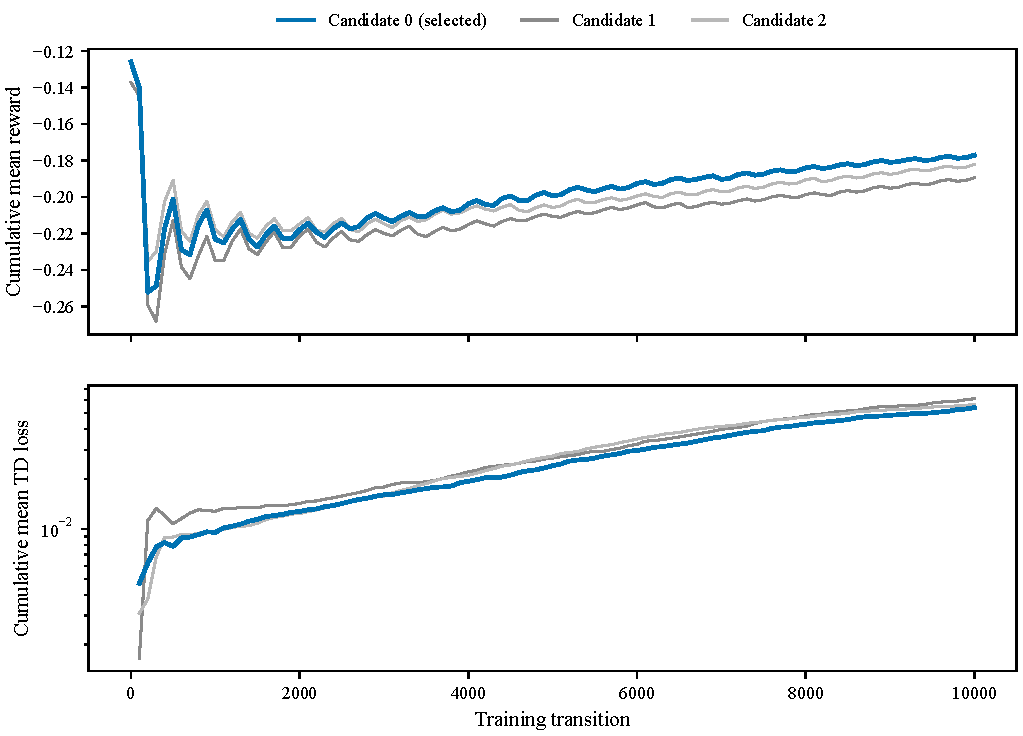
\includegraphics[width=\textwidth]{figures/v3-training-diagnostics.pdf}
  \caption{Development traces for the three v3 candidates.  Candidate 0 was
  selected by the predeclared validation rule and then frozen.  The lower panel
  uses a logarithmic axis for the cumulative mean squared temporal-difference
  (TD) loss.}
  \Description{Two vertically aligned line charts over ten thousand training
  transitions.  The top chart compares cumulative mean reward for three DQL
  candidates and highlights candidate zero.  The bottom chart compares their
  cumulative mean Bellman temporal-difference loss on a logarithmic scale.}
  \label{fig:v3-training-diagnostics}
\end{figure}

The cumulative mean TD loss rises for all three candidates after the early
updates, with all archived values finite and bounded. This is a training
diagnostic, not a convergence result. The target changes with the online
network and the states visited during training, so TD loss measures target
fit rather than model accuracy. Candidate selection used frozen-policy
validation and action coverage. The independent holdout supplies the
comparative performance results below.

\subsection{Independent Holdout Results}

Figure~\ref{fig:v3-scenario-reward} shows that outcomes differ across scenarios.
Frozen DQL has a higher return than the heuristic for
connection-count skew, tiered backlog, and client slowdown.  DQL and the
heuristic are indistinguishable in the pod-pressure scenario because both
select the same effective guarded response.  DQL also matches the static policy
under client slowdown: with client acknowledgement capacity as the bottleneck,
additional connection movement leaves the service-rate bottleneck unchanged.
These control cases identify when the policies provide equivalent outcomes.

\begin{figure}[!htbp]
  \centering
  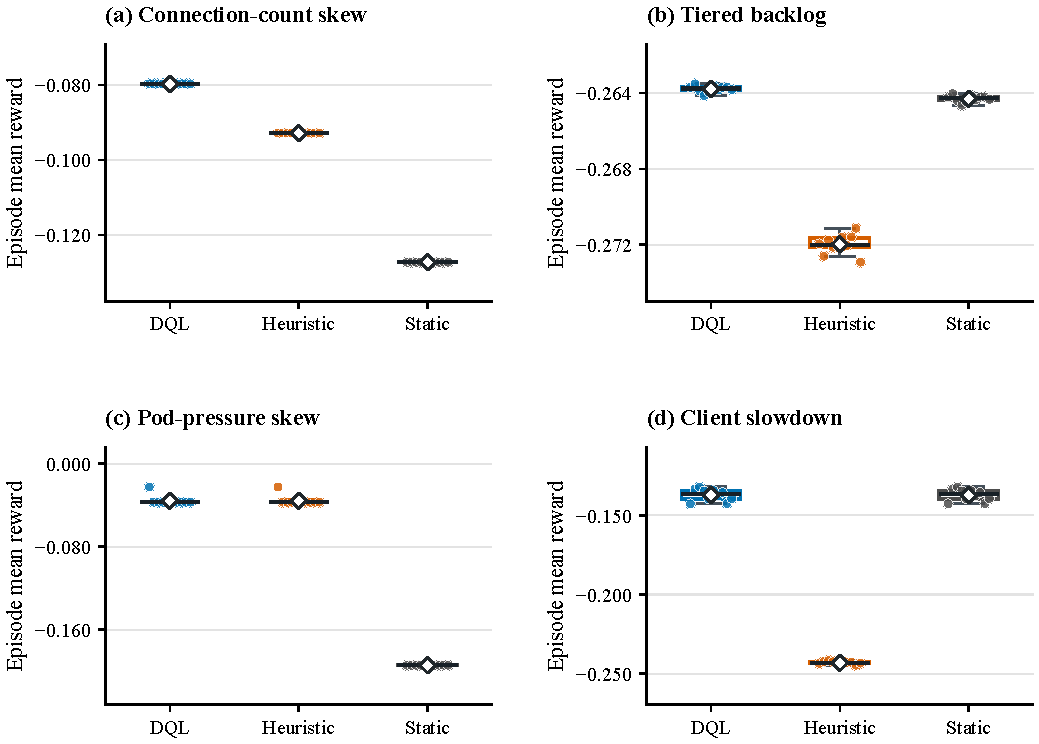
\includegraphics[width=\textwidth]{figures/v3-reward-boxplots.pdf}
  \caption{Holdout reward distributions for frozen DQL, heuristic, and static
  policies. Each panel contains ten paired seeds per policy. Boxes span the
  first and third quartiles, the central line is the median, whiskers extend
  to observations within 1.5 interquartile ranges, and diamonds mark means.
  Every episode is shown as a point, including observations beyond whiskers.
  Panels use separate vertical scales; higher reward is better.}
  \Description{Four box-and-point panels compare episode mean reward across
  connection-count skew, tiered backlog, pod-pressure skew, and client slowdown.
  Constant outcomes in the count-skew scenario collapse to horizontal lines.
  Frozen DQL has higher mean reward than the heuristic in three scenarios and
  equal reward in the pod-pressure scenario.}
  \label{fig:v3-scenario-reward}
\end{figure}

The boxes in Figure~\ref{fig:v3-scenario-reward} describe the distribution of
episode means, not the distribution of individual decision intervals. Horizontal
point offsets separate the ten observations without changing their rewards.
Collapsed boxes in the connection-count scenario reflect identical outcomes,
not missing data. Separate panel scales make the smaller spread in the tiered-backlog case
visible. The paired estimates below provide the statistical comparison, not
the visual height of a box.

Across all 40 paired episodes, frozen DQL improves mean reward over the
heuristic from $-0.1609$ to $-0.1291$.  The mean paired difference is $0.0318$
(bootstrap 95\% CI $[0.0191,0.0455]$), equivalent to a $19.8\%$ relative
benefit under Eq.~\eqref{eq:relative-benefit}; the paired standardized effect is
$d_z=0.729$, and the Holm-adjusted sign-flip $p$-value is below $0.001$.
Table~\ref{tab:v3-paired-effects} and Figure~\ref{fig:v3-paired-benefit} show
that this overall gain comes with tradeoffs.

\begin{table}[!htbp]
  \caption{Frozen DQL versus the heuristic on the independent v3 holdout.
  Positive benefit favors DQL.  CIs are paired-bootstrap intervals transformed
  by Eq.~\eqref{eq:relative-benefit}; $p_H$ is Holm-adjusted over 18 pooled
  metric-by-baseline tests.}
  \Description{Table listing DQL and heuristic means, direction-adjusted
  relative benefits with 95 percent confidence intervals, and Holm-adjusted
  paired sign-flip p-values for nine operational metrics.}
  \label{tab:v3-paired-effects}
  \centering
  \small
  \begin{tabular}{lrrrr}
    \toprule
    Metric & DQL & Heuristic & Benefit [95\% CI] (\%) & $p_H$ \\
    \midrule
    Mean reward & $-0.1291$ & $-0.1609$ & $19.8\ [11.9,28.3]$ & $<.001$ \\
    Backlog ratio & $0.1749$ & $0.2002$ & $12.7\ [-1.2,27.1]$ & $.095$ \\
    Conn.-subscription variance & $574.7$ & $5768.7$ & $90.0\ [61.0,120.8]$ & $<.001$ \\
    Conn.-backlog variance & $2.280\!\times\!10^{13}$ & $1.568\!\times\!10^{13}$ & $-45.4\ [-72.5,-22.6]$ & $.022$ \\
    Subscription imbalance & $0.0898$ & $0.4343$ & $79.3\ [59.1,99.5]$ & $<.001$ \\
    Backlog imbalance & $0.2194$ & $0.1638$ & $-34.0\ [-56.4,-13.6]$ & $.022$ \\
    Combined conn. imbalance & $0.1546$ & $0.2991$ & $48.3\ [33.8,63.8]$ & $<.001$ \\
    Pod pressure & $0.1878$ & $0.2051$ & $8.4\ [3.6,13.6]$ & $.022$ \\
    Throughput ratio & $0.2840$ & $0.2973$ & $-4.5\ [-7.1,-2.2]$ & $.022$ \\
    \bottomrule
  \end{tabular}
\end{table}

\begin{figure}[!htbp]
  \centering
  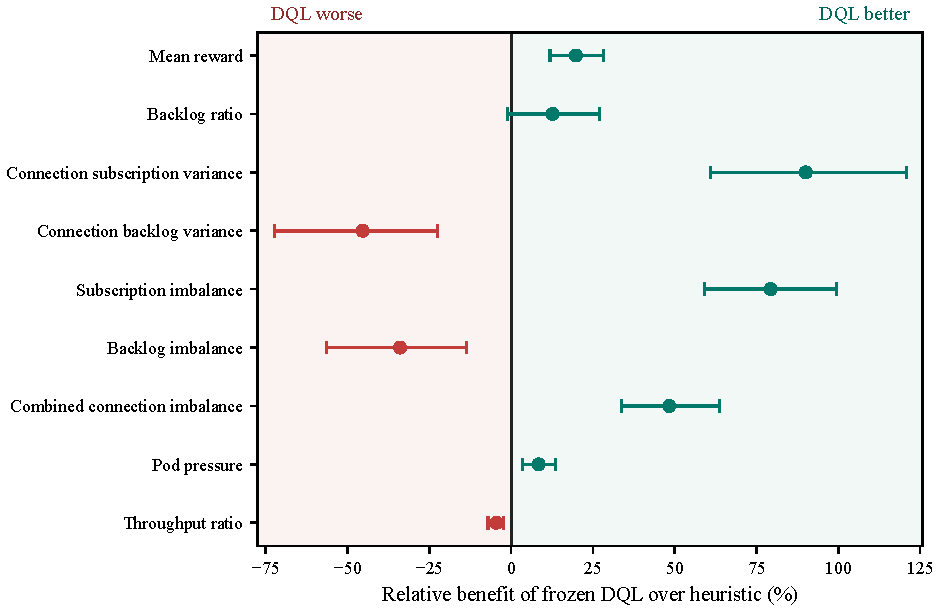
\includegraphics[width=\textwidth]{figures/v3-paired-benefit-forest.pdf}
  \caption{Direction-adjusted relative benefit of frozen DQL over the
  heuristic across 40 paired holdout episodes.  Points are mean effects and
  whiskers are paired-bootstrap 95\% confidence intervals.  Values right of
  zero favor DQL; values left of zero favor the heuristic.}
  \Description{Horizontal forest plot for nine metrics.  DQL improves reward,
  connection subscription variance, subscription imbalance, combined
  connection imbalance, and pod pressure.  Its backlog ratio interval crosses
  zero, while connection backlog variance, backlog imbalance, and throughput
  favor the heuristic.}
  \label{fig:v3-paired-benefit}
\end{figure}

The largest benefit is a $90.0\%$ reduction in connection-level subscription
variance, consistent with the design objective of moving subscriptions away
from overloaded persistent connections.  Subscription imbalance falls by
$79.3\%$, combined connection imbalance by $48.3\%$, and mean pod pressure by
$8.4\%$.  Mean backlog ratio is $12.7\%$ lower, but its interval crosses zero
and the adjusted test is not significant ($p_H=.095$).  Conversely, DQL has
$45.4\%$ higher connection-backlog variance, $34.0\%$ higher normalized backlog
imbalance, and $4.5\%$ lower throughput than the heuristic.  The scalar reward
still favors DQL because its configured penalties place substantial weight on
subscription pressure and combined imbalance. The holdout therefore identifies
a multi-objective advantage for DQL and a queue-drainage advantage for the
heuristic.

\begin{figure}[!htbp]
  \centering
  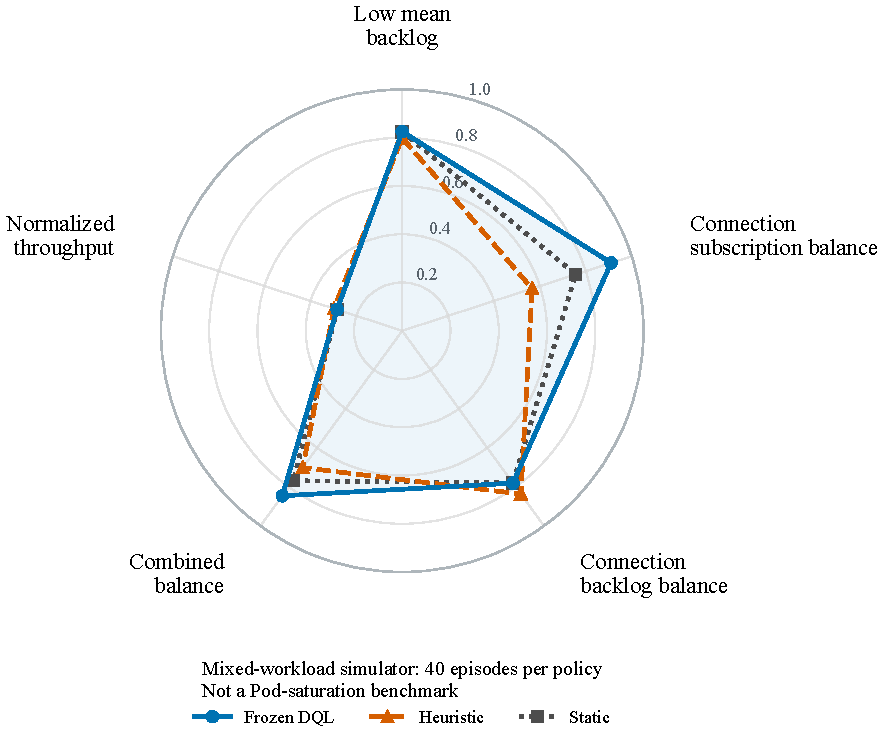
\includegraphics[width=\textwidth]{figures/v3-operational-radar.pdf}
  \caption{Mixed-workload simulator profiles, not a Pod-saturation benchmark,
  across 40 paired holdout episodes per policy. Subscription balance is
  measured across client connections, not across all Pods. All axes use a
  fixed zero-to-one scale with larger values preferred. Backlog and imbalance
  costs are displayed as one minus their mean normalized value; throughput
  retains its recorded normalized value. The profiles are descriptive, not
  an additional weighted score or significance test.}
  \Description{A five-axis radar chart compares frozen DQL, heuristic, and
  static policies. DQL extends farther on subscription and combined balance;
  the heuristic extends farther on backlog balance and throughput. All profiles
  use the same normalization and the full zero-to-one radial range.}
  \label{fig:v3-operational-radar}
\end{figure}

Figure~\ref{fig:v3-operational-radar} summarizes these tradeoffs without mixing
raw variances with event rates. For policy $\pi$ and a normalized cost metric $x_v$,
the plotted coordinate is $1-\bar{x}_{\pi,v}$; the throughput coordinate is
$\bar{x}_{\pi,\mathrm{throughput}}$. Here each mean covers the same 40 episodes,
with ten episodes from each scenario. No observed minimum or maximum is used
to stretch an axis. DQL's stronger subscription and combined balance coexist
with the heuristic's stronger backlog balance and throughput. Polygon area
has no statistical interpretation, and the combined-balance axis is derived
from the two imbalance components rather than being an independent outcome.
Uncertainty and paired comparisons remain those in
Table~\ref{tab:v3-paired-effects} and Figure~\ref{fig:v3-paired-benefit}.

This pooled profile characterizes the mixed workloads; Pod saturation is
evaluated separately. The
connection-count-skew workload has no arrivals or initial backlog and therefore
contributes zero throughput for all policies. In the pod-pressure workload,
all policies serve the offered traffic with essentially zero residual backlog;
their throughput is therefore equal despite different Pod pressure. The
client-slowdown workload is limited by client acknowledgement capacity.
Count balance and recovery of overloaded-Pod bandwidth are therefore separate
endpoints. The saturated scale-out comparison is
reported separately in Figures~\mainref{fig:scaleout-backlog-recovery}
and~\ref{fig:scaleout-violin-distributions}.

The distinction is operational, not merely graphical. Equal subscription
counts can leave every persistent socket on the same saturated Pod, and moving
idle subscriptions does not redistribute queued work. Conversely, moving
backlogged subscriptions to a Pod with spare service capacity can raise
aggregate throughput, provided client ACK capacity and shared Queue or network
limits do not become the bottleneck. In the scale-out experiment, the initial
connection counts and backlogs are already balanced
($V_u^N(0)=V_u^G(0)=0$), yet all ten sockets terminate on one Pod. Migration
across Pods raises measured simulator throughput from 58,000 to 219,762 events/s
(3.79 times). Thus, the throughput-recovery evidence is the stressed placement
comparison in Section~\mainref{sec:scaleout-recovery}. Connection-balance scores
describe a different property. The Oracle Cloud preload pair in
Section~\ref{sec:ttl-preload-results} measures expiry and ACK completion with
the migration guard held at stay.

The comparison with static control isolates the benefit of rebalancing under
concentrated load. In the 1,600-subscription pod-pressure scenario, three of
four active connections initially terminate on the same pod. Static placement
therefore retains mean pod pressure $1.0125$, whereas DQL promotes a guarded
probe target and reduces it to $0.2176$, a $78.5\%$ reduction. The corresponding
paired reward improvement is $0.1588$ (95\% bootstrap CI
$[0.1573,0.1617]$). In the connection-count-skew scenario, DQL reduces mean
connection subscription-count variance from $6{,}250.0$ to $2{,}298.7$
($63.2\%$) and improves mean reward by $0.0475$. Across all four scenarios,
pooled mean reward improves by $0.0517$ relative to static placement. The
scenario plot also identifies cases where DQL and static placement are equal.
The paired analysis assigns each measured gain to its workload, keeping the
concentrated-load and tiered-backlog results separate.


\subsection{Action-Contract Validation}

The v3 policy passed the declared subscription-count, backlog-rebalancing,
and migration coverage gates. The expanded v4--v6 studies tested all five
interventions and fault guards. None passed every learned-action coverage
gate, although the v6 candidates all passed the safety scenarios. These
completed development studies do not supply additional holdout performance
estimates. Appendix~\ref{app:action-diagnostics} retains their full results,
including the scripted test of the corrected scale-up contract.

\subsection{Adverse-Probe Promotion Ablation}
\label{sec:adverse-probe-ablation}

The retained probe is a candidate endpoint, not an instruction to migrate.
To isolate this distinction, we registered a paired mechanism experiment before
the confirmatory run. In every episode, the probe was set to reach the pod with the highest
initial pressure. The deployment mask evaluated the concrete
source--target pair and rejected $a^{\mathrm{mig}}$ whenever its projected
pressure improvement was below 0.01. The primary ablation then bypassed that
mask for exactly one interval, moved the highest-backlog non-target connection
to the adverse pod, and returned control to the same frozen DQL checkpoint.
Thus, \emph{Frozen DQL} and \emph{DQL + forced promotion} differ only by that
initial override and its subsequent state consequences. \emph{Blind
promotion} makes the same move and then stays; \emph{Static} never changes the
initial placement; and the guarded heuristic uses the same feasibility mask as
DQL.

For total backlog $B(t)$ in the evaluated subscription population over $T$
decision intervals, the primary endpoint is
the normalized trapezoidal backlog area
\begin{equation}
  \mathrm{AUC}_{B}=\frac{1}{T}
  \sum_{t=1}^{T}\frac{B(t-1)+B(t)}{2B(0)}.
  \label{eq:normalized-backlog-auc}
\end{equation}
It measures how much work remains queued over time. Lower values indicate
earlier drainage. The statistical unit is the environment seed, not an interval. The
primary cohort uses 30 previously unused paired seeds and 1,200 subscriptions.

\begin{figure}[!htbp]
  \centering
  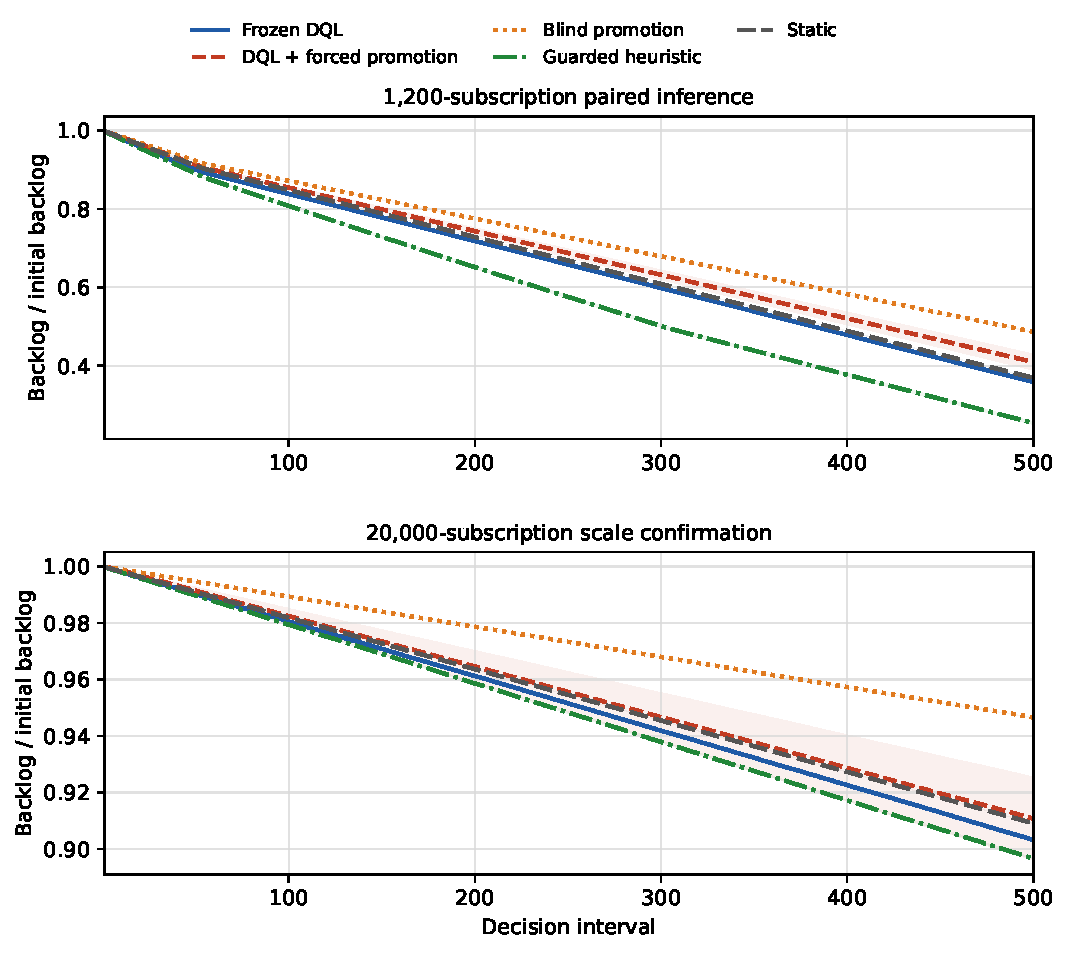
\includegraphics[width=\textwidth]{figures/backlog_trajectories.pdf}
  \caption{Mean normalized backlog trajectories for the adverse-probe
  ablation. Shaded bands are descriptive 95\% normal-approximation intervals
  across paired seeds. The upper panel contains the 30-seed inference cohort;
  the lower panel contains the five-seed 20,000-subscription scale
  confirmation. The forced-promotion policy resumes the same frozen DQL
  controller after the interval-zero override.}
  \Description{Two vertically aligned backlog-ratio line charts compare frozen
  DQL, the same DQL after one forced adverse promotion, blind promotion, a
  guarded heuristic, and static placement. Guarded DQL remains below forced,
  blind, and static placement, while the guarded heuristic drains fastest.}
  \label{fig:adverse-probe-trajectories}
\end{figure}

Each episode runs for 500 intervals. Paired mean differences use 10,000
bootstrap resamples and one-sided sign randomization with 100,000 sign vectors;
Holm adjustment covers the four named baselines. The action mask rejected the
adverse migration in all 30 primary and all five scale-confirmation
environments.

In the primary cohort, guarded DQL attains mean $\mathrm{AUC}_{B}=0.66046$,
compared with 0.68938 after the forced promotion. The paired difference is
$-0.028918$ (95\% CI $[-0.039444,-0.019073]$), a 4.19\% reduction relative to
the forced-promotion ablation. The raw one-sided randomization $p$-value is
$1.0\times10^{-5}$ and the Holm-adjusted value is
$4.0\times10^{-5}$. Guarded DQL also reduces backlog AUC by 9.34\% relative to
blind promotion and by 1.41\% relative to static placement. Its final backlog
ratio is 0.35875, compared with 0.40936, 0.48584, and 0.36864, respectively.
The throughput differences have the same direction: DQL delivers 43.02
million messages, 2.35 million more than the forced-promotion ablation and
5.91 million more than blind promotion.

\begin{table}[!htbp]
  \caption{Adverse-probe ablation outcomes. Backlog AUC and final backlog are
  normalized by initial backlog; lower is better. Throughput is cumulative over
  500 intervals. The 20k cohort is descriptive ($n_{\mathrm{ep}}=5$).}
  \Description{Table comparing mean normalized backlog area, final backlog
  ratio, cumulative throughput, and pod pressure for five policies in the
  1,200-subscription inference and 20,000-subscription scale cohorts.}
  \label{tab:adverse-probe-outcomes}
  \centering
  \resizebox{\textwidth}{!}{%
  \begin{tabular}{llrrrr}
    \toprule
    Cohort & Policy & Backlog AUC & Final ratio & Throughput (M) & Mean pressure \\
    \midrule
    1.2k inference & Frozen DQL & 0.66046 & 0.35875 & 43.02 & 0.5873 \\
    1.2k inference & DQL + forced promotion & 0.68938 & 0.40936 & 40.66 & 0.6100 \\
    1.2k inference & Blind promotion & 0.72853 & 0.48584 & 37.11 & 0.5874 \\
    1.2k inference & Guarded heuristic & 0.59104 & 0.25384 & 47.90 & 0.5941 \\
    1.2k inference & Static & 0.66993 & 0.36864 & 42.56 & 0.5870 \\
    \midrule
    20k confirmation & Frozen DQL & 0.95155 & 0.90316 & 97.05 & 0.7877 \\
    20k confirmation & DQL + forced promotion & 0.95556 & 0.91076 & 91.16 & 0.7884 \\
    20k confirmation & Blind promotion & 0.97323 & 0.94645 & 63.50 & 0.7875 \\
    20k confirmation & Guarded heuristic & 0.94828 & 0.89658 & 102.15 & 0.7883 \\
    20k confirmation & Static & 0.95452 & 0.90903 & 92.50 & 0.7875 \\
    \bottomrule
  \end{tabular}%
  }
\end{table}

\begin{figure}[!htbp]
  \centering
  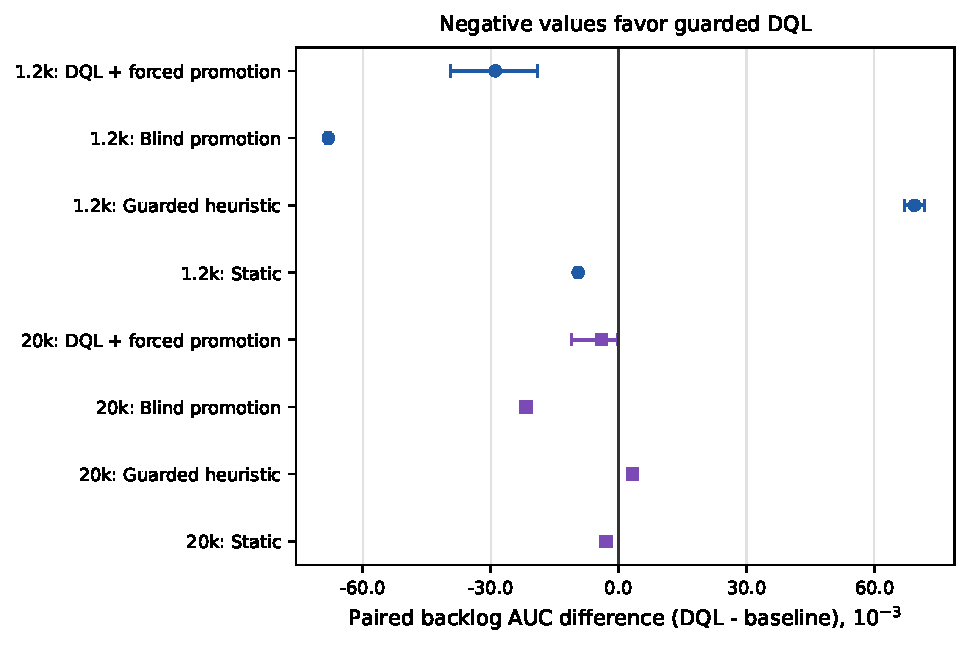
\includegraphics[width=\textwidth]{figures/paired_auc_effects.pdf}
  \caption{Paired normalized backlog-AUC differences between guarded DQL and
  each baseline. Negative values favor DQL; whiskers are paired-bootstrap 95\%
  confidence intervals. Squares denote the descriptive 20,000-subscription
  cohort.}
  \Description{Horizontal forest plot showing DQL below forced promotion,
  blind promotion, and static placement in both cohorts. The heuristic points
  lie above zero, showing that it has lower backlog area than DQL.}
  \label{fig:adverse-probe-effects}
\end{figure}

The heuristic provides an important comparison. Its primary-cohort backlog AUC
is 0.59104, so DQL is 11.75\% higher (paired difference 0.069419, 95\% CI
$[0.066977,0.071826]$). The action records explain the difference. Across 15,000
primary decision intervals, the heuristic executes 2,286 backlog-rebalancing
actions, whereas DQL executes 175 backlog and 175 subscription-count moves and
otherwise stays. In the 20k cohort, the heuristic uses all 625 interventions for backlog rebalancing. DQL splits
625 interventions almost evenly between 315 backlog and 310 subscription-count moves. The backlog-specific measure therefore favors the heuristic, which makes
more backlog-focused moves.
The ablation establishes the benefit of guarding probe promotion; the
backlog-focused heuristic retains the stronger queue-drainage result.

The 20,000-subscription cohort retains the requested four equal groups:
5,000 subscriptions at 100,000 queued messages, 5,000 at 50,000, 5,000 at
5,000, and 5,000 at zero, totaling 775 million initial messages. Guarded DQL
reduces backlog AUC by 0.42\% relative to forced promotion, 2.23\% relative to
blind promotion, and 0.31\% relative to static placement, while remaining
0.34\% above the heuristic. The forced-promotion paired interval lies below
zero, but its exact one-sided $p=0.0625$ and Holm-adjusted $p=0.125$ reflect the
five-seed sample. We consequently treat this cohort as scale confirmation, not
as a second inferential test. The maximum normalized message-conservation
residual over all 175 episodes is $1.031\times10^{-14}$; this verifies simulator
accounting but does not establish loss-free production handoff.


\subsection{Reproducibility and Study Scope}

\paragraph{Reviewer artifact access.}
The accompanying supplementary archive, \texttt{reviewer-evidence.zip},
contains episode-level simulator CSVs, declared protocols, original aggregate
analyses, the frozen 21--32--6 checkpoint, and identifier-free live summaries.
Its README gives the file map and exact offline commands. A Python 3.9+
standard-library script verifies the checksum manifest, checks paired cohort
coverage, recomputes policy means and selected effect sizes, and reconciles
the loaded trial's reported subscription and ACK totals. A separate inference
option evaluates the saved network without transport access or model updates.
The archive supports reanalysis and checkpoint inspection; it does not expose
corporate credentials, raw event payloads, private endpoint identifiers, or
the proprietary service source. It is not a complete independent deployment
rerun. Provenance records distinguish unchanged measurements from redacted
local-path metadata.

The manuscript bundle contains the exact v3 aggregate CSV files, v3--v6 JSON
protocols and summaries, the adverse-probe protocol and episode-level outputs,
and the scripts that regenerate every figure in this section. The
larger private evidence archive additionally records source-file SHA-256 hashes,
frozen-checkpoint hashes, raw episode rows, and a recursive checksum manifest.
The implementation test suite contains unit tests for state construction,
action masks, replay, checkpoint persistence, migration state transitions, and
fault guards, together with a Java STOMP fixture. At the source revision used
for this manuscript, all 267 tests pass, including the four adverse-probe
evaluator tests, cap-restoring scale-up tests, and legacy-policy rejection
tests.

The recovery study includes 20,000 subscriptions and four modeled pods;
the earlier four-scenario holdout contains up to 1,600 subscriptions. These
are simulator measurements with explicit workload and service assumptions.
The v4--v6 all-action studies ended at their development coverage gates and
are reported as diagnostics, separate from holdout performance. The Oracle
Cloud cluster experiment in Section~\mainref{sec:mumbai-experiment} measures
20,000-subscription topology and ten live handoffs using existing queued
events rather than the simulator's paired, controlled workloads. The
backlog-recovery effect sizes therefore apply to the stated simulator. The
Oracle Cloud measurements establish execution of the corresponding
connection-replacement mechanism in Kubernetes.
The additional loaded scale-out run in Section~\mainref{sec:live-dql-scaleout}
records three selective DQL handoffs and 8,000 acknowledged STOMP deliveries
for 1,000 subscriptions. It uses a fixed client-processing delay and bounded
publication, and supplies functional handoff evidence rather than a matched
throughput effect size.


